\documentclass[preprint,10pt,authoryear,review]{elsarticle}
%\documentclass[final,8pt,authoryear,twocolumn]{elsarticle}

%% Use the option review to obtain double line spacing
%% \documentclass[preprint,review,12pt]{elsarticle}

%% Use the options 1p,twocolumn; 3p; 3p,twocolumn; 5p; or 5p,twocolumn
%% for a journal layout:
%% \documentclass[final,1p,times]{elsarticle}
%% \documentclass[final,1p,times,twocolumn]{elsarticle}
%% \documentclass[final,3p,times]{elsarticle}
%% \documentclass[final,3p,times,twocolumn]{elsarticle}
%% \documentclass[final,5p,times]{elsarticle}
%% \documentclass[final,5p,times,twocolumn]{elsarticle}

%% if you use PostScript figures in your article

%% or use the graphicx package for more complicated commands
\usepackage{graphicx}
\graphicspath{{Figures/}}
%% or use the epsfig package if you prefer to use the old commands
\usepackage{epsfig}
%% The amssymb package provides various useful mathematical symbols
\usepackage{amssymb,amsmath}
%% The amsthm package provides extended theorem environments
\usepackage{amsthm}
\usepackage{algorithm}
\usepackage{algpseudocode}
\usepackage{textcomp}
\usepackage{subcaption}


%% The lineno packages adds line numbers. Start line numbering with
%% \begin{linenumbers}, end it with \end{linenumbers}. Or switch it on
%% for the whole article with \linenumbers after \end{frontmatter}.
%\usepackage{lineno}

%% natbib.sty is loaded by default. However, natbib options can be
%% provided with \biboptions{...} command. Following options are
%% valid:

%%   round  -  round parentheses are used (default)
%%   square -  square brackets are used   [option]
%%   curly  -  curly braces are used      {option}
%%   angle  -  angle brackets are used    <option>
%%   semicolon  -  multiple citations separated by semi-colon
%%   colon  - same as semicolon, an earlier confusion
%%   comma  -  separated by comma
%%   numbers-  selects numerical citations
%%   super  -  numerical citations as superscripts
%%   sort   -  sorts multiple citations according to order in ref. list
%%   sort&compress   -  like sort, but also compresses numerical citations
%%   compress - compresses without sorting
%%
%% \biboptions{comma,round}

% \biboptions{}
\usepackage{hyperref}
\usepackage{color}
\usepackage{textcomp}
\usepackage{multirow}
\usepackage{float}
\usepackage{amsmath}

\journal{Computer and Chemical Engineering}

\begin{document}

\begin{frontmatter}
\title{Accelerating multi-dimensional population balance model simulations with a highly scalable framework on GPUs.}


\author[label1]{Chaitanya Sampat}
\author[label1]{Yukteshwar Baranwal}
\address[label1]{Chemical and Biochemical Engineering, 
Rutgers University, Piscataway, NJ, USA - 08854}
\author[label1]{Rohit Ramachandran\corref{cor1}}
\ead{rohitrr@soemail.rutgers.com}
\cortext[cor1]{Corresponding author}
%\ead[url]{pslrutgers.com}

\begin{abstract}
Population Balance models (PBMs) are widely used in pharmaceutical industry to simulate
and optimize the granulation process. Prediction of time evolution of the distribution 
of the particulate properties using these PBMs, is very important in understanding
key dynamics. However, with an increase in the number of components and phases in 
a particulate mixture, complexity of a PBM increases. This leads to multi-dimensional 
matrix calculations potentially requiring significant computational power. Solving 
such a system of equations with a traditional central processing unit (CPU) would 
be intractable.
%thus there is a need of a parallel framework which can help decrease 
%the simulation time. 
%Over the past decade, graphical process units (GPUs) are increasingly being 
%used for computation. 
This study focuses on the development of an algorithm to parallelize the nested 
loops inside the PBM via a GPU framework. The developed PBM was parallelized 
specifically for NVIDIA GPUs as it was written in CUDA C/C++. The contribution of 
communication time between the CPU and GPU in the code contributed to less than 1\% of 
the total run time leading to a maximum speedup of about 12 over the serial code being 
achieved on the GPU. The speed up reported for the GPU PBM was about 2x the PBM 
code on multi-core configuration on a desktop computer. The speed improvements 
are also reported for various CPU \& GPU architectures and configurations.
%The speed improvements were also tested with various combinations in 
%discretization of the granulator geometry and threads used for calculations. 
\end{abstract}

\begin{keyword}
%% keywords here, in the form: keyword \sep keyword
Population Balance Model \sep GPU \sep Parallel Computing \sep Granulation \sep MPI \sep CUDA
%% MSC codes here, in the form: \MSC code \sep code
%% or \MSC[2008] code \sep code (2000 is the default)
\end{keyword}

\end{frontmatter}

%\begin{linenumbers}
%% main text
\section{Introduction}
\label{secIntro}
Over the past decade, Population Balance Models (PBMs) have been used to predict 
several industrial processes \citep{ramkrishna2014}. The population balance equation is 
simply a number conservation of particles which regulate the behavior of the entire system.
PBMs can be divided into several external and internal coordinates, which can add 
bring more accuracy to the model. Deriving accurate equations to determine these rate of change 
of these  internal coordinates requires precise empirical co-relations from 
experimental data. Another method used to a mechanistic kernel can be introduced in these 
models to make them more accurate \citep{Barrasso2015cerd}. 
The PBM accuracy can also be improved by incorporating larger number of solid bins 
inside the PBM. The increase in the number of solid bins leads to an increase in 
calculations for each time step, leading to a higher simulation times. The calculations 
increase by a factor of $n^4$ where n being the number of solid bins. An accurate model 
which incorporates higher number of solid bins as well as includes a mechanistic kernel 
in its calculations is expected to be sluggish to simulate and could take several hours 
to complete. Such models and their solving techniques are not viable to be used in real 
time system control. Thus, there is a need to improve the time it takes to simulate the 
model.

The advancement of computers and its peripherals in recent years have led to a great increase in 
computational resources leading to faster simulations. The recent central processing unit (CPU) 
now contain various cores thus making it possible to run multiple processes in parallel. 
In order to take advantage of a highly parallel framework, large number of cores are needed 
which may not be possible in a personal desktop and a supercomputer cluster needs to be used.
Another computer peripheral that can to be used to run a highly parallel code is the computer's 
graphic processing unit (GPU)~\citep{Prakash2013b}. These GPUs contain thousands of compute 
cores that can be used run tasks in parallel. Thus, a desktop equipped with a GPU could 
compute the same results as a CPU code on supercomputers in lesser amount of time as seen 
in Section \ref{secResults}. With the launch of Compute Unified Device Architecture (CUDA), 
NVIDIA made it easier to use GPUs for general parallel programming in an approach usually 
termed as general purpose computing on GPUs (GPGPUs).

Various chemical industries like detergent, food, pharmaceutical, fertilizers, catalyst encounter 
particulate processing daily. 
These processes constitute to about $50\%$ of the world's chemical production \citep{seville1997}.
In the pharmaceutical industry, particulate processes are widely used to increase 
the size of the granules, improve flow-ability, increase yield strength etc. One of 
major processes in among these to increase the granule size is granulation. 
Granulation is the process in which fine pharmaceutical powder 
blends are converted to larger granules using a liquid or a dry binder \citep{Chaturbedi2017}. 
These larger granules help in better flow ability and strength to these mixtures 
aiding further processing. 

Understanding the dynamics of the continuous granulating system is vital for its smooth 
operation and to reduce the amount of waste generated in the development phase. The Food 
and Drug administration (FDA) has also been promoting a similar initiative with its 
Quality by Design (QbD) and Process Analytically Tools (PAT) principles~\citep{sen2014} 
\citep{FDAPAT2004}. Thus, a process model for the system becomes an integral part 
of the development phase. A model which predicts the bulk mechanical properties of the 
mixture as well as a particle size distribution (PSD) is required. 


The main objective of this work is to develop a highly scalable framework for to simulate 
PBMs on GPUs. This framework would be independent of the type of kernels as well as number 
of spatial compartments as well as the number of solid bins used. The framework would be 
universal and would be able to run of different NVIDIA GPUs without the need for any changes. 
The number of threads that the PBM will use depends upon the size of the problem as well as 
the number of cores available on the GPU. This code was developed in NVIDIA CUDA C/C++. 
A similar code was also developed on C++ to be run on the CPU which has limited scalability 
due to number of CPU cores available on desktop computer. This work also enables the use of 
desktop computers to obtain numerical solutions to computation intensive tasks rather than 
relying on supercomputers for quicker results.


%
%In the present study, a mechanistic multi-dimensional PBM was developed such that it was not 
%only accurate but also scalable since the number of solid bins could be changed to alter its 
%behaviour. This model was developed in C++ to be run on CPUs. This C++ model was parallelised 
%using Message Parsing Interace (MPI) which is parallel application programming interface (API). 
%This model was developed NVIDIA GPUs and was parallelized using the CUDA toolkit. The timings of 
%the simulations were then compared for each of these cases. The scalability of the GPU based code 
%was also tested to obtain speed improvements over serial CPU code.


\section{Background and previous works}
\label{secBkgd}
\subsection{Population balance modeling in Granulation}

Population balances have been successful in 
predicting physical phenomena occurring in granulation such as aggregation, breakage and 
consolidation. These models predict how groups of distinct entities inside the pharmaceutical 
powder behave on a bulk scale due to process parameters over time of granulation. A
general representation of the model is:

\begin{align}
\frac{ \partial}{\partial t}&F(\textbf{v},\textbf{x},t) + \frac{\partial}{\partial 
\textbf{v}}[F(\textbf{v},\textbf{x},t)\frac{d\textbf{v}}{dt}(\textbf{v},\textbf{x},t)] 
+ \frac{\partial}{\partial \textbf{x}}[F(\textbf{v},\textbf{x},t)\frac{d\textbf{x}}{dt}
(\textbf{v},\textbf{x},t)] \notag\\
    &= 
\Re_{formation}(\textbf{v},\textbf{x},t)+\Re_{depletion}(\textbf{v},\textbf{x},t)
+\dot{F}_{in}(\textbf{v},\textbf{x},t) -\dot{F}_{out}(\textbf{v},\textbf{x},t) 
\label{eqn:bkgd_pbm_general} 
\end{align}

where $\textbf{v}$ is a vector of internal 
coordinates.  $\textbf{v}$ is commonly used to describe the solid, liquid, 
and gas content of each type of particle. The vector $\textbf{x}$ represents 
external coordinates, usually spatial variance. $F$ represents the 
number of particles present inside the system, $\dot{F}_{in}$ 
and $\dot{F}_{out}$ is the rate of particles coming in and going out the 
system respectively. $\Re_{formation}$ and $\Re_{depletion}$ are the rate of 
formation and depletion due various phenomena.

Granulation is the process of engineering granules from pharmaceutical powder blends 
with the addition of liquid or solid binders. This process is usually carried out 
to obtain granules with a certain PSD,  bulk densities and other physical properties
~\citep{Barrasso2015cerd}.
There are about 3 rate processes that occur due the addition of a liquid binder to the 
powder mixture are wetting and nucleation, consolidation and aggregation, and breakage 
and attrition~\citep{sen2014}. To understand the process dynamics and control these 
process, population balance equations have been accepted as a relevant methodology \citep{Immanuel2005}.

In a high shear granulator, the particles are rendered wet 
when they come in contact with the liquid binder, which also aids in granule formation due to 
liquid bridges. These granules can also break into smaller fragments due to shear stresses, 
compressive and tensile forces that are exerted on to the system due the impeller, 
particle-particle interactions and particle-wall interactions.


Prediction of PSDs and other particle bulk properties is highly dependent on 
the kernels used to describe the sub-processes inside granulation. Identification 
of a kernel that describes the sub-processes suitably is of the essence in this model 
since they are not only size dependent but also time dependent. Recently, various 
mechanistic kernels have been developed that help capture the micro-mechanics of the 
system, which help in better prediction of the final particle size \citep{Barrasso2015processes}. 
Several of these kernels maybe dependent on other physical simulations such as Discrete 
Element Model (DEM) to obtain certain information about the microscopic phenomena 
occurring inside the system.


\subsection{Parallel Computing}
Computing with its current infrastructure has become an important tool in science. 
Parallel computing is one of the more extensively used type of computing used by scientists 
to perform simulations. It is the process of splitting of larger calculations into 
many smaller processes executed concurrently \citep{Almasi1989}. This type of execution 
helps achieve large speed gains overs simulations run on a single core in a serial manner.
The computational task can be decomposed by various means to help simulate the system 
in a reasonable amount of time. The simulation problem can be decomposed either 
at the task level or at the data level. Task parallelism involves each process to 
behave distinctively from another as they would each be performing different operations. 
These multiple operations could be performed on a single data set or on multiple data 
sets, known as multiple instruction single data (MISD) and multiple instruction 
multiple data (MIMD) respectively. On the other hand, data parallelism 
involves the distribution of data across various processes which usually perform same set of 
operations on the data \citep{solihin2015}. This type of parallelism is known 
as single instruction multiple data (SIMD). MIMD and SIMD can also 
be combined in certain systems, thus decreasing the simulation times further.

\subsection{GPU based parallel computing}
Traditionally, large parallel jobs needed to be run on supercomputers which had thousands 
of cores, but these are require special components making them expensive.
Graphic processing unit (GPU) were initially used for vector calculations to support 
graphics inside a computer system. But, lately GPU manufacturers have started to promote them 
general computing as well. This form of computing has been gaining popularity among scientists 
to accelerate simulations \citep{kandrot2011}. These GPUs comprise of a 
massively parallel architecture with hundreds to thousands of computational cores 
which can have thousands of active threads running simultaneously \citep{keckler2011}. 
This means that GPUs have large cWomputing potential the GPU computing can be exploited using parallel programming languages 
such as OpenCL and CUDA. 

CUDA is an application programming interface (API) developed by NVIDIA \citep{NVIDIA2012} 
that enables users to program parallel code for execution on the GPU. This framework is an 
extension implemented on top of C/C++ or Fortran. Parallel code for the GPU is written 
as kernels, which theoretically are similar to functions or methods in traditional 
programming languages. As several parts of the code need to executed only once during a simulation, 
only few sections of the code can be written in terms of kernel while the remaining has 
to be executed in serial on the CPU of the system. The \texttt{nvcc} 
compiler from the CUDA toolkit prioritizes the compilation of these kernels before 
passing the serial section of the code to the native C/C++ compiler inside the system. 
There are three main parallel abstractions that exist in CUDA are grids, blocks and 
threads \citep{santos2013}. Each CUDA kernel is executed in a serial manner during the execution 
of the program unless specified, where the kernels can be run in parallel using CUDA 
streams. Each kernel executes as a grid which in turn consists of various blocks which 
are consistuted by various threads. This thread-block-grid hierarchy helps obtain fine 
grained data level and thread level parallelism. An illustration of this hierarchy is 
observed in Figure \ref{fig:bkg_gpu_arch}.

Another important aspect related to GPU parallelization is the data communication between the threads. 
The GPU consists of various memory modules with different access limitations as shown in Figure 
\ref{fig:bkg_gpu_arch}. The threads inside each block can communicate with each other using the 
shared memory. This memory is local to the block where these threads exist i.e. they are not 
accessible by threads from other blocks. In addition to the shared memory each thread has its 
own local memory where local/temporary variables for each kernel can be saved to them. 
The threads from different communicate with each other using the global memory which is visible to 
all blocks inside the GPU at the cost of higher communication times. Accessing of data from the 
local memory is the fastest for a thread and its slows down as we move towards shared block memory 
and the least for accessing data from the global GPU memory. 


\begin{figure}[h]
\centering
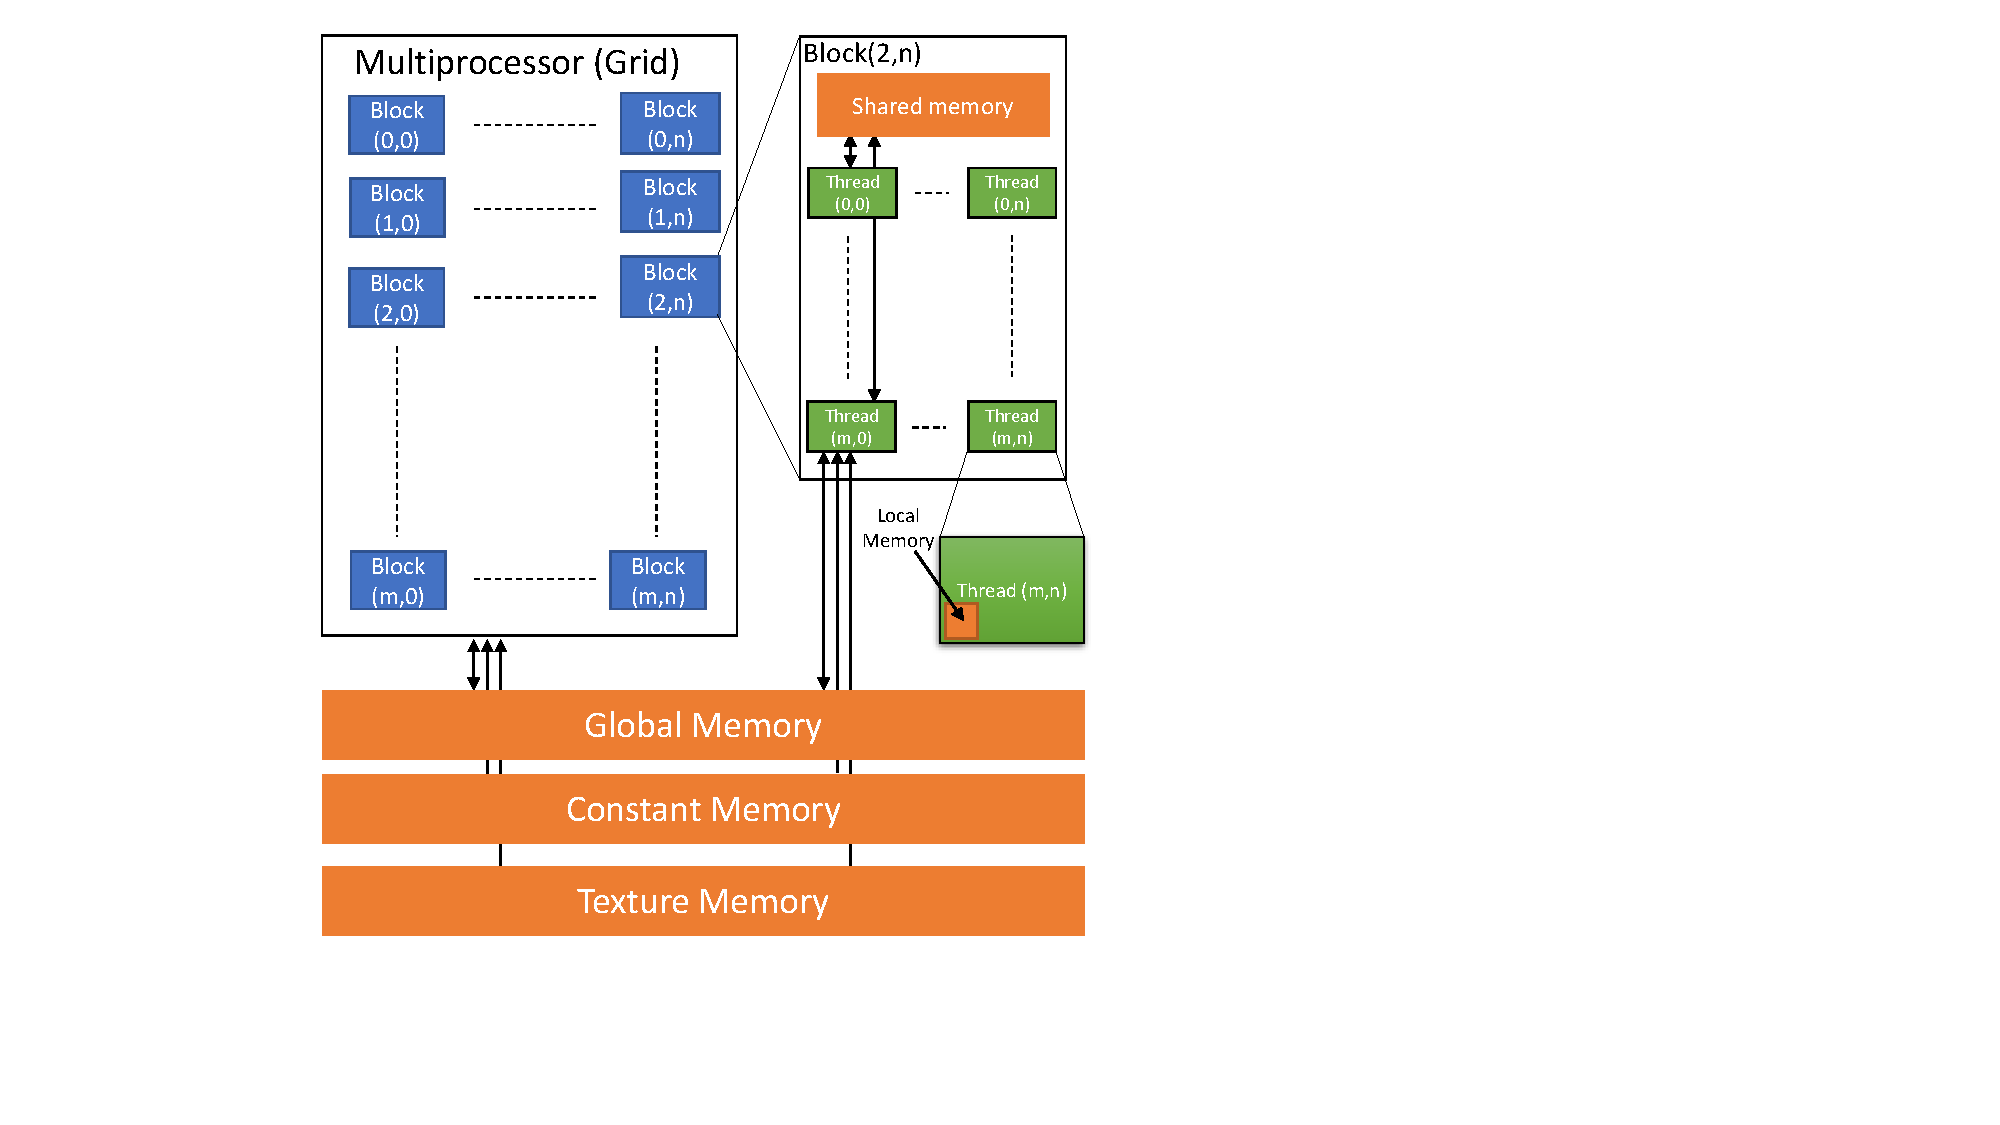
\includegraphics[scale=0.75]{gpu_arch_new.pdf}
\caption{The parallel structure matrix inside the GPU and the various memories associated 
with each structure.}
\label{fig:bkg_gpu_arch}
\end{figure}


\subsection{Previous parallelized PBM works}
PBMs have known to be been computationally intensive especially ones with larger internal 
coordinates and higher dimensions. Thus, several researchers have made attempts to increase 
the speed of these simulations. \cite{Gunawan2008} developed a parallelization technique 
for a high-resolution finite volume solution of the PBM. The parallel algorithm presented by 
\cite{Gunawan2008} in their scale up studies for the PBM upto 100 cores achieved good 
parallel efficiency, implying the algorithm's effectiveness. The study was not performed for 
higher number of dimensions inside the PBM. This study also suggested that an algorithm 
with a shared memory model could help improve simulation speeds further. A hybrid memory model 
was implemented by \cite{Bettencourt2017} to obtain speed improvements of about 98\% from the 
serial code. This implementation took into account both Message Parsing Interface (MPI) as well 
as Open Multi-processing (OMP). A similar PBM parallelization approach was also undertaken in 
\citep{Sampat2018} and a speed up of about 13 was obtained. The reduction in speed was attributed 
to the use of dynamic arrays used in their PBM framework to accommodate the hybrid nature of the 
model being used. 

Algorithms to parallelize the PBM codes on GPU have been studied briefly by \cite{Prakash2013b} 
using the inbuilt MATLAB's parallel computing toolbox (PCT). This study was able to achieve 
good speed ups but could have been higher if the code had been implemented in native 
programming languages such as C or FORTRAN. Other works that have used GPU acceleration 
to improve computation times for their population balance simulations include those from 
various other chemical engineering processes such as crystallization \citep{Szilagy2016}, 
combustion \citep{Shi2012} , multiphase flow \citep{santos2013} , coagulation dynamics 
\citep{Xu2015}. Previous literature lacks the discussion of adaptation of the parallel 
algorithm scaling when several model parameters are changed at once. 


\section{Method and implementation}
\label{secMethods}
\subsection{PBM implementation}
The overall population balance equation used in our algorithm looked like \citep{ramkrishna2014}:
\begin{align}
\frac{d}{dt}F(s_i,l,g,x,t)&=\Re_{agg}(s_i,l,g,x,t)+\Re_{break}(s_i,l,g,x,t)\notag\\ 
&+\dot{F}_{in}(s_i,l,g,x,t)-\dot{F}_{out}(s_i,l,g,x,t)
\label{eqn:mthds_pbm_overall} 
\end{align}
where, $F(s_i,x)$ represents the number of solid particles of type i being studied in each spatial 
compartment $x$ of the granulator. The rate of aggregation $\Re_{agg}(s_i,x)$ 
and the rate of breakage $\Re_{break}(s_i,x)$ determines the rate at which particles density
changes within different size classes. The rate of particles entering, $\dot{F}_{in}(s_i,x)$ 
and exiting, $\dot{F}_{out}(s_i,x)$, the spatial compartment due to particle transfer also 
affects their number in each size class. The rate of change of internal liquid volume in each 
particle can be calculated as: 

\begin{align}
\frac{d}{dt}F(s_i,x)&l(s_i,x)= 
\Re_{liq,agg}(s_i,x)+\Re_{liq,break}(s_i,x)+\dot{F}_{in}(s_i,x)l_{in}(s_i,x)\notag\\
&-\dot{F}_{out}(s_i,x)l_{out}(s_i,x)+F(s_i,x)\dot{l}_{add}(s_i,x)
\label{eqn:mthds_pbm_rate} 
\end{align}
where, $l(s_i,x)$ is the internal liquid volume in each particle with ${s_i}$ as the 
solid volume for solid type 1 in the spatial compartment $x$. 
$\Re_{liq,agg}(s_i,x)$ and $\Re_{liq,break}(s_i,x)$ are the rates at which liquid is transferred 
between size classes due to aggregation and breakage respectively. $l_{in}(s_i,x)$ 
and $l_{out}(s_i,x)$ are the internal liquid volumes of the particles entering and exiting 
the spatial compartment. $l_{add}(s_i,x)$ is the volume of liquid acquired 
by each particle in the compartment at every time step due to external liquid addition.
Similarly, the rate of change of gas volume is calculated using the following equation: 

\begin{align}
\frac{d}{dt}F(s_i,x)g(s_i,x)&= 
\Re_{gas,agg}(s_i,x)+\Re_{gas,break}(s_i,x)+\dot{F}_{in}(s_i,x)g_{in}(s_i,x)\notag\\
&-\dot{F}_{out}(s_i,x)g_{out}(s_i,x)+F(s_i,x)\dot{g_cons}(s_i,x)
\label{eqn:mthds_pbm_gas_agg} 
\end{align}
where, $g(s_i,x)$ is the gas volume of each particle with solid volumes of $s_i$ 
in the spatial compartment $x$. $\Re_{gas,agg}(s_i,x)$ and $\Re_{gas,break}(s_i,x)$ are 
the rates of gas transferred between size classes due to aggregation and breakage respectively. 
$g_{in}(s_i,x)$ and $g_{out}(s_i,x)$ are the gas volume of the particles entering and 
leaving the spatial compartment respectively. $\dot{g_cons}(s_i,x)$ represents the volume of 
gas particles formed due to process of consolidation occurring inside the system. The 
rate of aggregation, $\Re_{agg}(s_i,x)$ in Equation \ref{eqn:mthds_pbm_overall} is 
calculated as \citep{Chaturbedi2017}:

\begin{align}
\Re_{agg}(s_i,x)&= \frac{1}{2}\int _0^{s_i} \int _0^{s_i'} 
\beta(s_i',s_i-s_i',x)F(si',x)F(s_i-s_i',x)ds_ids_i'\notag\\ 
&- F(s_i,x)\int _0^{s_{max_i}-s_i} 
\beta(s_i,s_i',x)F(s_i',x)ds_i'
\label{eqn:mthds_R_agg}
\end{align}
where, $\beta(s_i, s_i',x)$ is the aggregation kernel and is expressed as a 
function of collision frequency ($C$) and collision efficiency ($\psi$). Further 
information on the model can be found in \ref{app:aggKernel}.

Similarly, the breakage rate can be expressed as follows:
\begin{align}
\Re_{break}(s_i,x)  = \int_0^{s_{max_i}} & \notag
K_{break}(s_1',s_2',x)F(s_1',s_2',x)ds_i' \\ &  - K_{break}(s_i,x)F(s_i,x)ds_i
\label{eqn:mthds_pbm_breakage_geneq}
\end{align}   
where, $K_{break}(s_i,x)$ is the breakage kernel. The formulation for the breakage 
kernel is discussed in more detail in \ref{app:breakKernel}.

The rate of increase of liquid volume of inside a particle, 
$\dot{l}_{add}(s_i,x)$ is expressed as:

\begin{align}
\dot{l}_{add}(s_i,x) = \frac{(\sum_i(s_i)(\dot{m}_{spray})}{m_{solid}(x)}
\label{eqn:mthds_liq_addn_rate}
\end{align}
where, $\sum_i(s_i)$  is the total solid volume of the particle; $\dot{m}_spray$ is the 
rate of external liquid addition and $m_{solid}$ is the total amount of solid present in the compartment.
%
%The rate of decrease in gas volume per particle due to consolidation is calculated using the 
%following expression \citep{Verkoeijen2002}:
%
%\begin{align}
%\dot{g}_{cons}(s_i,x)=&c (\nu_{impeller})^{\omega}V(s_i,x)\frac{(1-\epsilon_{min})}{s} 
%\notag \\ 
%& \left[g(s_i,x)+l(s_i,x) -(s_1+s_2)\frac{\epsilon_{min}}{1-\epsilon_{min}}\right]
%\label{eqn:mthds_rate_gas_vol_part}
%\end{align}        
%
%where, $c$ and $\omega$ are the consolidation constants; $v_{impeller}$ is the impeller 
%rotational speed; $\epsilon_{min}$ is the minimum porosity; 

Particle transfer rate, $\dot{F}_{out}(s_i,x)$ in Equation \ref{eqn:mthds_pbm_overall} 
is calculated as:

\begin{align}
\dot{F}_{out}(s_i,x) = \dot{F}(s_i,x)\frac{\nu_{compartment}(x)*dt}{d_{compartment}}
\label{eqn:mthds_f_out_dot_part_trans_rate}
\end{align}

where, $\nu_{compartment}(x)$ and $d_{compartment}$ are respectively the average 
velocity of particles in compartment $x$ and the distance between the mid-points 
of two adjacent compartment, which is the distance particles have to travel to 
move to the next spatial compartment. $dt$ is the time-step.

A finite difference method was used to solve the developed system of ordinary differential 
equations (ODEs) \citep{Barrasso2015cerd}. The numerical integration technique used 
was first order Euler integration as it is commonly used for speed improvements as while 
having minimal impact on accuracy \citep{Barrasso2013}. In order to avoid numerical 
instability due to the explicit nature of the Euler integration, Courant-Friedrichs-Lewis 
(CFL) condition must be satisfied~\citep{courant1967}. For our PBM model, time-step was 
calculated at each iteration such that, the number of particles leaving a particular bin 
at any time is less than the number of particles present at that time \citep{Ramachandran2010}.

\subsection{MPI implementation}
The message parsing interface (MPI) parallel implementation of the PBM was 
focused towards equal distribution of the task and memory. The implementation 
used in this work differs from the hybrid implementation used by \citep{Bettencourt2017}
and \citep{Sampat2018} as only MPI was used to parallelize the code. It 
was pointed by \citep{Sampat2018} that open message parsing (OMP) does not 
provide significant speed improvements due to limitations with usage of 
dynamic vectors which are essential for such a system. Thus, the OMP 
implementation was avoided which also meant that lesser number of cores 
would be required. The focus of this study to localize the computation power 
rather than depend on supercomputers/clusters. MPI was used for message passing 
from one core to another as well as all the calculations  
were performed on the same MPI core. As pseudo code has been presented in Algorithm 1 
to illustrate the distribution of tasks. For each time step, a MPI process is responsible 
for a certain section of the problem, usually a spatial chunk inside the geometry 
(also referred to as compartment).  



Simulations for this study were performed on a computer with an Intel Core i7-7700K 
processor clocked at 4.2GHz and 32 GB of RAM. For maximum performance while 
data reading and writing a SSD was used. GCC version 7.4 with openMPI 2.0 
was used to compile the parallel C++ code.

\begin{algorithm}
     \scriptsize
     \caption{CPU-based Parallel Population Balance Model}
     \label{alg:CPUparallelPBM}
     \begin{algorithmic}[1]
     \Procedure{PBM}{$N_{Comp}$,$N_{MPI}$}\Comment{$N_{Comp}$ is the number of compartments}
     \State \texttt{Divide $N_{Comp}$ in $N_{MPI}$}
     \While{$t < t_{final}$}
     \For{$\forall n_{Comp}$ in 1 MPI process}
     \State \texttt{Calculate $\Re_{aggregation}$ for solid bins $s_1$,$s_2$}
     \State \texttt{Calculate $\Re_{breakage}$ for solid bins $s_1$,$s_2$}
     \State \texttt{Calculate $n_{particles}$ using Euler's method}
     \EndFor
     \State \texttt{Collect $n_{particles}$ from $N_{MPI}$}\Comment{Master process collects all data}
     \State \texttt{Calculate $timestep$ using \textit{CFL} condition}
     \State \texttt{$t_{new} = t + timestep$ }
     \EndWhile
     \EndProcedure
     \end{algorithmic}
 \end{algorithm}   




%To obtain the most optimal parallel performance, when solving the PBM, workloads 
%were distributed in a manner which took into account the shared and distributed 
%memory aspects of the clusters, the PBM was being run on. To parallelize the model 
%in a way which could take advantage of shared memory but still effectively run 
%across a distributed system both MPI and OMP were implemented. One MPI process 
%was used per CPU core and one OMP thread was used per CPU core, as 
%Bettencourt et al. (2017) found it resulted in the  performance. MPI was 
%used for message passing from one node to another while OMP was used for 
%calculations on each node that could be efficiently solved using a shared 
%memory system.‎ An algorithm in the form of pseudo code is presented in the 
%Appendix illustrating how the calculations are distributed and carried out 
%during the simulation. For each time step, the MPI processes are made 
%responsible for a specific chunk of the spatial compartments. Then each 
%OMP thread, inside of each MPI process, is allocated to one of the cores 
%of multi-core CPU the MPI process is bound too. The OMP threads divide up 
%and compute $R_agg$. After $R_agg$ is calculated the MPI processes calculate 
%the new PSD value for their chunk at that specific time step, Ft,c. The 
%slave processes send their Ftc to the master processes which collects them 
%into the complete Ft,all. The master process then broadcasts the Ft, all 
%value to all slave processes. This decomposition of the data into‎ 
%different CPUs and further into various threads is illustrated in 
%Figure 3-4.‎ A crucial feature of the PBM is that the current PSD (Ft,all) 
%value is used to compute a new‎ time step size for the next iteration. 
%This means all of the MPI processes need to have the same‎ dynamic time 
%step size at each iteration for the calculations to be properly carried 
%out in parallel.‎ Since the completely updated Ft, all value is shared 
 %before calculating a new time step each process‎ will have the same Ft, 
%all value. As a result each process calculates the same size for the 
%new time‎ step.‎ Since the DEM informed PBM code required dynamic size 
%increase for the data structure due‎ to different number of particles 
%being present in the DEM simulation, the PBM code developed‎ used the 
%Standard Template Library containers and their features available 
%in C++ 11 and later.‎ It requires intel v17.0.2 (GCC 5.3+) or later 
%for compilation. Since this module was not present on‎ the Stampede,
%the execution of the PBM was done on the newer Stampede2 supercomputer. 
%Each‎ of the compute node of the cluster consists of Intel Xeon Phi 7250 
%(“Knights Landing") which has‎ 68 cores on a single socket clocked at 1.4 GHz, 
%with 96 GB of DDR4 RAM. Each of the cores‎ consists of 4 hardware threads. 
%The simulations were then run by varying the number of MPI‎ processes from 
%1 to 16 and the number of OMP threads from 1 to 8, thus, using a maximum of 128‎ cores.

\subsection{GPU implementation}
NVIDIA’s CUDA toolkit extends the C language such that user defined functions 
called kernels can be created to be run on the GPU. These kernels can be 
executed several number of times in parallel using large number of threads. A thread is 
sequence if programmed instructions that can be managed by the computer’s 
scheduler. A kernel depending upon the dimensions of the data can execute 
instructions in 1-D, 2-D or 3-D thread blocks. The kernel can also launch 
multiple thread blocks at once, thus increasing the number of parallel 
process executions known as grid. Similar to a thread block, a grid can 
be up to 3-D depending upon the data under study.
The code execution was split between the CPU (also called host) and GPU 
(also called device). Time sensitive calculations as well as mixed data 
calculations were handled on the CPU with a single core, while the more 
computationally intensive tasks were distributed on to the GPU using 
kernels. Like in the CPU parallelization, the geometry was split into 
multiple compartments. These compartments in turn formed the number of 
blocks inside each GPU kernel. The number of solids used helped formed 
the threads in each of these blocks. The work flow of the execution can 
be found in Figure \ref{fig:mtd_gpu_imp}. The orange arrows in Figure 
\ref{fig:mtd_gpu_imp} indicate the 
transfer of data from the CPU memory to the GPU memory and vice-versa 
whereas the blue arrows indicate the sections of the code that is sent 
to the GPU for parallel execution.

\begin{figure}
\centering
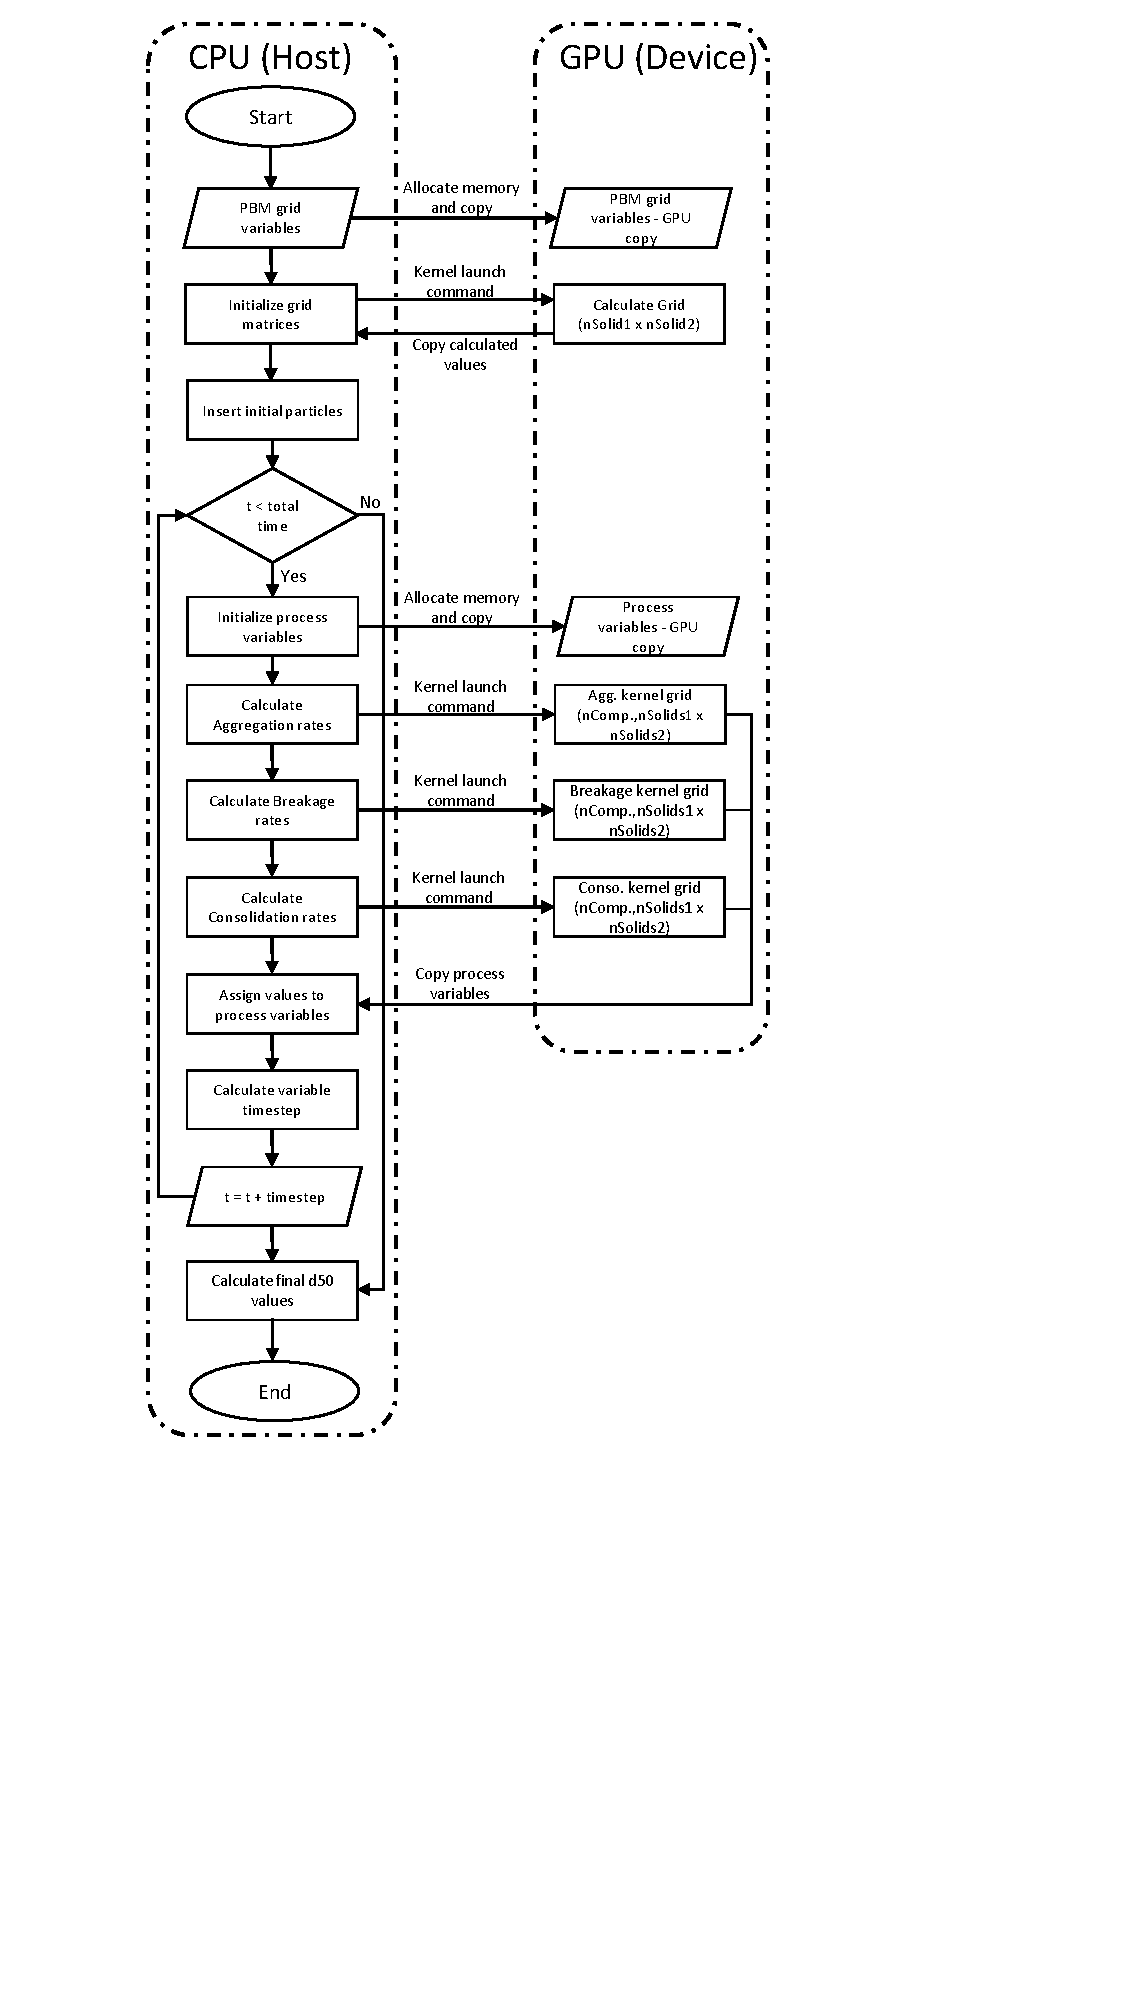
\includegraphics[scale=0.8,trim=200 250 300 200]{GPU_flowchart.pdf}
\caption{Workflow of the GPU code indicating data transfers and execution timeline of the code.}
\label{fig:mtd_gpu_imp}
\end{figure}


\begin{algorithm}
     \scriptsize
     \caption{GPU-based Parallel Population Balance Model}
     \label{alg:GPUparallelPBM}
     \begin{algorithmic}[1]
     \Procedure{PBM}{$N_{Comp}$}\Comment{$N_{Comp}$ is the number of compartments}
     \State\texttt{Copy initial variables from CPU memory to GPU memory}
     \State \texttt{GPU initial calculation kernel call from CPU}\Comment{Performed on GPU}
     \State \texttt{Divide $N_{Comp}$ in $N_{blocks}$}
     \State \texttt{Copy back initial values to the CPU RAM}
     \While{$t < t_{final}$}
	 \State \texttt{Copy time-dependent process variables from CPU to GPU RAM}
     \State \texttt{GPU aggregation rate kernel call from CPU}
     \State \texttt{Calculate $\Re_{agg}$ for solid bins $s_1$,$s_2$}\Comment{Performed on GPU}
	 \State \texttt{GPU aggregation rate kernel call from CPU}     
     \State \texttt{Calculate $\Re_{breakage}$ for solid bins $s_1$,$s_2$}\Comment{Performed on GPU}
     \State \texttt{Calculate $n_{particles}$ using Euler's method}
     \State \texttt{Copy back process rate data back to the CPU RAM}
     \State \texttt{Calculate $timestep$ using \textit{CFL} condition}\Comment{Performed on CPU}
     \State \texttt{$t_{new} = t + timestep$ }
     \EndWhile
     \State \texttt{Clear GPU memory}
     \EndProcedure
     \end{algorithmic}
 \end{algorithm}

\section{Results and discussions}
\label{secResults}
\subsection{Performance metrics}
Parallel efficiency of an algorithm can be tested either by strong scaling 
where the problem size remains the same and number of processing elements 
are increased or by weak scaling where the number of processing elements 
remain the same and the problem size is increased. In this study, the 
number of processing units were limited due to the architecture of the 
GPU and the CUDA C++ code developed did not utilize more than one GPU 
during execution. Thus, a soft scaling approach was preferred in such a 
scenario. The parallel performance of a code is usually measured in 
terms of on ratio of time taken to solve the run the simulations on one 
core to the time taken to run the simulation on N cores. It is depicted in
Equation \ref{eqn:result_parallelefficiencyWeak}, where $t_1$ is the time taken 
to the run the problem on one core where as $t_N$ is the time taken to 
run the problem on N cores.

\begin{align}
\ Speedup = \frac{t_1}{t_N}
\label{eqn:result_parallelefficiencyWeak}
\end{align}

The problem size was varied by increasing the number of compartments inside 
the PBM. This in turn increased the total number of calculations performed 
without increasing the amount of work that needed to be performed by each 
processing unit (core). The number of cores required during the simulation 
on the GPU was determined by the product of the number of compartments and 
the number of solid bins for each solid type used. Thus, the number of GPU 
cores used in this study varied from 256 cores for 1 compartment to 8192 
for 32 compartments.

Parallelization of code can lead some deviation of the calculations from 
the serial execution. This discrepancy in calculation can be attributed to 
the difference in the precision of the cores of the CPU or GPU being used. 
This change in precision can lead to a small error in one timestep 
percolating to produce results that can drastically different from the serial 
code. To check the validity of the presented algorithm a relative least sum 
of squares error was calculated as shown in Equation \ref{eqn:result_rSSe}:


\begin{align}
\label{eqn:result_rSSe}
rSSE = {\sum}_{i=0}^{t_{end}‎}\frac{(d_{50_{serial_i}}-d_{50_{parallel_i}})^2}{N} \qquad
\end{align}

The $rSSE$ was calculated for the algorithm considering the single core MPI 
solution as the base and determining the error values wrt to this simulation.
The error for each of the case can be found in Figure \ref{*}. The average error 
for the GPU was less than $x\%$ which is an acceptable range. Thus, making the 
solutions from the algorithm quicker with a very small loss in accuracy.

\textbf{INSERT ERROR PLOT. }

\subsection{Algorithm performance on a desktop GPU}
The desktop configuration used for these studies comprised of a Intel $i7-7700K$  
CPU clocked at $4.5$ GHz with $32$ GB DDR4 RAM and a NVIDIA Quadro $P4000$ GPU. 
The NVIDIA Quadro GPU used had 1792 CUDA cores with 8 GB of GDDR5 RAM. 
CUDA version 9.0 paired with GCC 7.3 was used to the run the desktop GPU simulations 
with Ubuntu 18.04 operating system (OS).


Each GPU consisted of several streaming multi-processors(SM) which help 
distribute the problem to the 1792 cores inside the GPU. Once the calculations  
pass from the CPU to the GPU, the SMs take over and allocate work to the GPU in 
blocks of $32$ threads each. This distribution was found to be one of the major 
bottlenecks especially when control was handed over from the CPU to the GPU. 
This leads to a significant time delay if the amount of calculation to be 
performed by the GPU is low and the control exchanges are more common. 
The number of solid bins for the 2 different types of solids used were $16$, 
this meant that there was a maximum of $65,536$ calculations that needed to 
be performed for each time step for each compartment. While, the
number of calculations increased to over 2 million per time step when the number of 
compartments was increased to $32$. SMs divide these calculations in blocks 
of 32 threads and send it to the cores for calculations which accounts for some 
overheard time during the simulation. This overhead is present for each timestep, 
which can be compensated by the number of calculations running in parallel on 
the GPU. The PBM was run for $90$ seconds which included $45$ seconds of mixing 
and 45 seconds of liquid addition. The algorithm performance was tested by soft scaling 
the problem by changing the number of compartments from $1$ and doubling them in 
each simulation until the number of compartments reached $32$. Figure \ref{fig:res_gpu_timings} 
shows the time taken these simulation. It can be seen that the amount of time taken 
for the simulation remains almost constant till the number of compartments reaches $8$, 
followed by an increase in the time taken as the number of compartment are increased 
further to $32$. According to parallelization procedure used the cores utilized to run the 
code is directly proportional to the number of compartments and the number of solid bins 
present in the problem. The constant time is a result of the problem size being smaller than 
the Quadro $P4000$'s 1792 CUDA core, i.e. the algorithm was not able to utilize all the 
CUDA cores till the compartment number was $8$. Since the algorithm uses about $256$ cores 
to simulate each compartment, the cores would not suffice once the compartment number reaches 
$16$ and the SMs would have to wait to distribute the calculation to cores once 
initially allocated calculations are finished. This wait time leads to the increase in the 
time of simulations as seen in the case for $16$ and $32$ compartments. 

\begin{figure}[h]
\centering
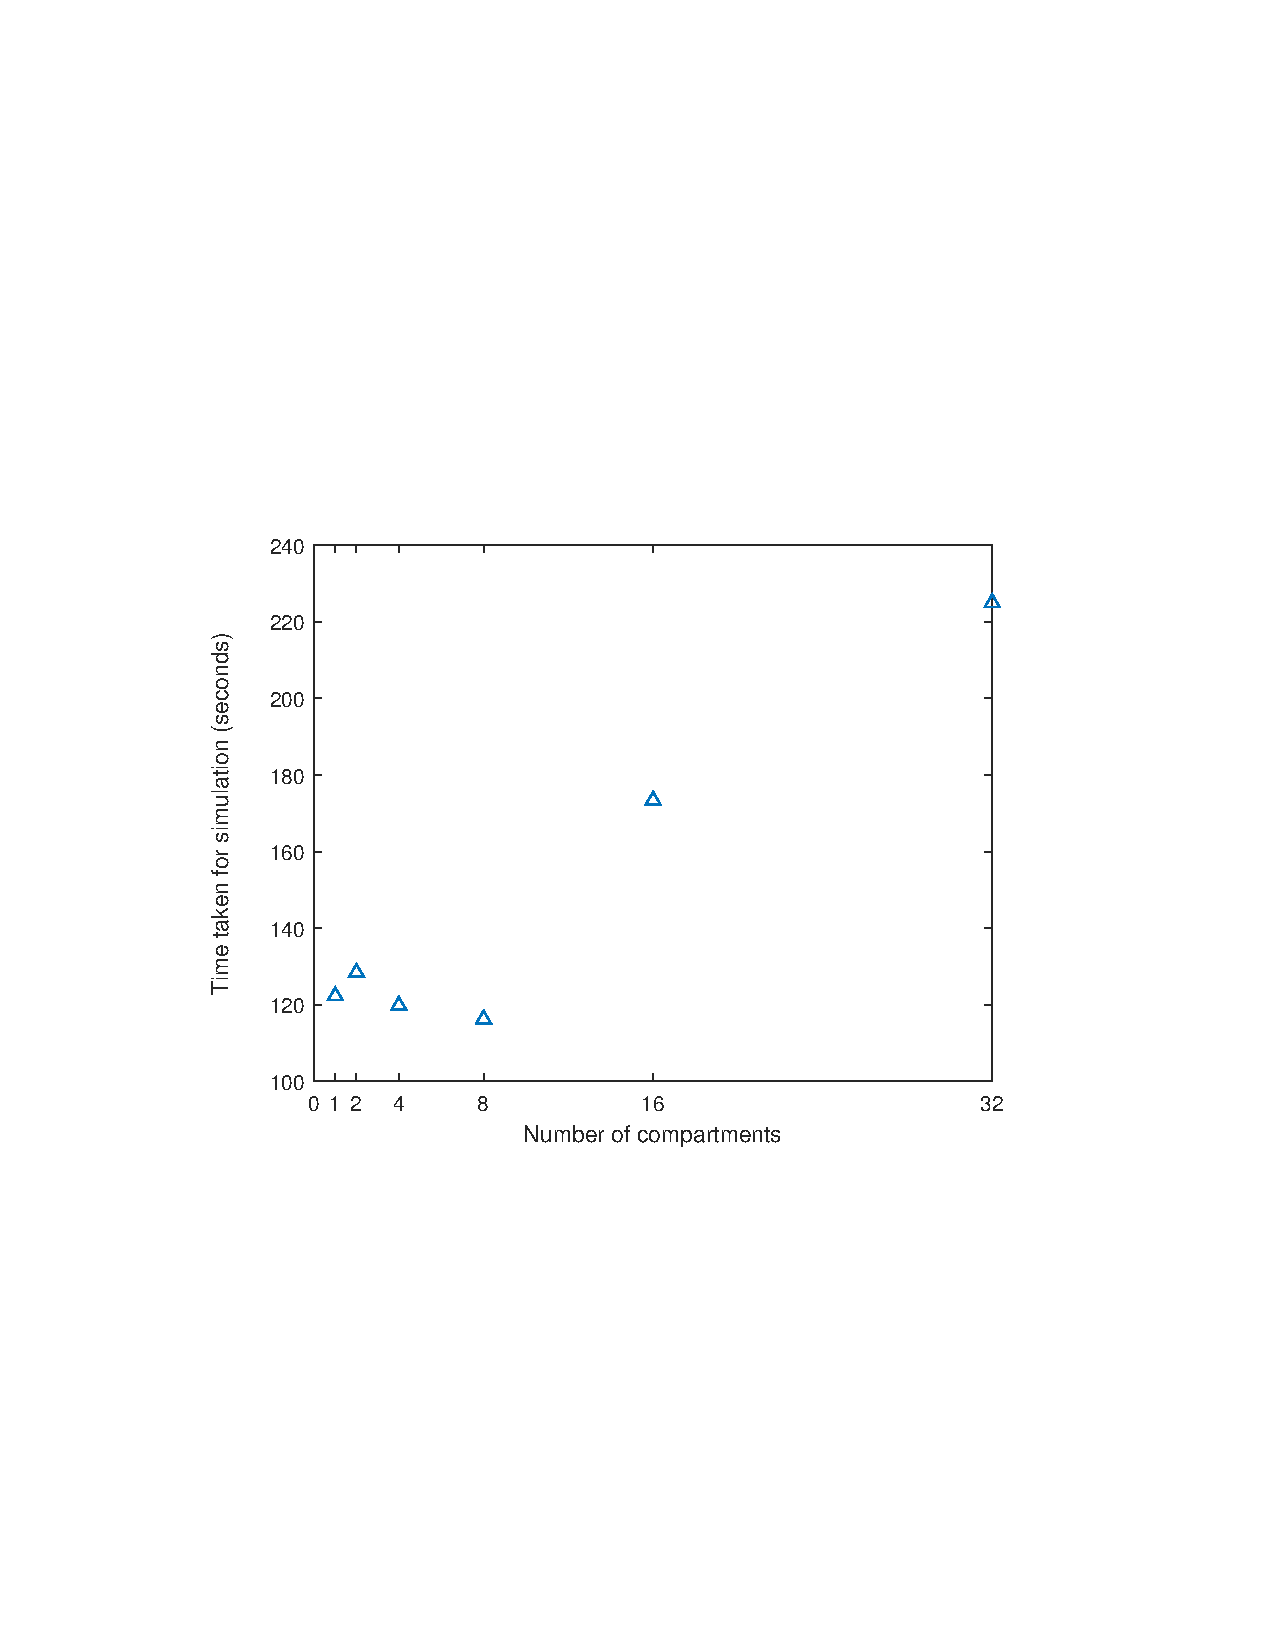
\includegraphics[scale=0.7,trim=110 220 120 220, clip]{desktopgputiming.pdf}
\caption{Time taken to complete 90 seconds of PBM simulation with varying number of compartments 
on NVIDIA Quadro P4000 GPU}
\label{fig:res_gpu_timings}
\end{figure}


The above argument was supported by the profile of the code that was obtained using NVIDIA's
inbuilt code profiler $nvprof$. Code profiling is an important step in algorithm development. 
The profiler results can be varied based on the options chosen to obtain the parameters being 
studied. In this case, API calls and GPU activity were exported to understand the performance 
bottlenecks and those sections of the code were rectified to improve the speed of the algorithm.
The profiler was executed for each case and it was observed that aggregation kernel calculations 
took the most time for execution followed by the breakage kernel. Consolidation kernel 
and other calculations comprised of less than $1$\% of execution time. The other parameter 
studied was the number of times each API was summoned by the code and the time spent. API 
calls included the synchronization of threads working inside the GPU device, memory allocation 
for arrays, etc. Each thread inside the GPU operates independently,
thus all threads may not be at the same line of code at a given moment of time, thus some threads 
finish calculations before others. The time taken to synchronize these threads required the most 
amount of time during the execution of the code. When such an API is called by the code 
further execution of the code is paused until all the threads of the GPU are in the same 
line of code. This accounted for $99$\% of the total other API call time. This indicated that there 
were not many places where the code could have been optimized further since synchronization 
statements were only added before calculations where complete array of data was required. 
If further reduction in these statements was undertaken, it would lead to data loss and 
possibly incorrect final calculated particle size distribution. A comparison of times taken 
by each process in the simulations is shown in Figure \ref{fig:res_profile_pie}. A similar 
distribution of times was observed for all simulations on the GPU.

\begin{figure}[h]
\centering
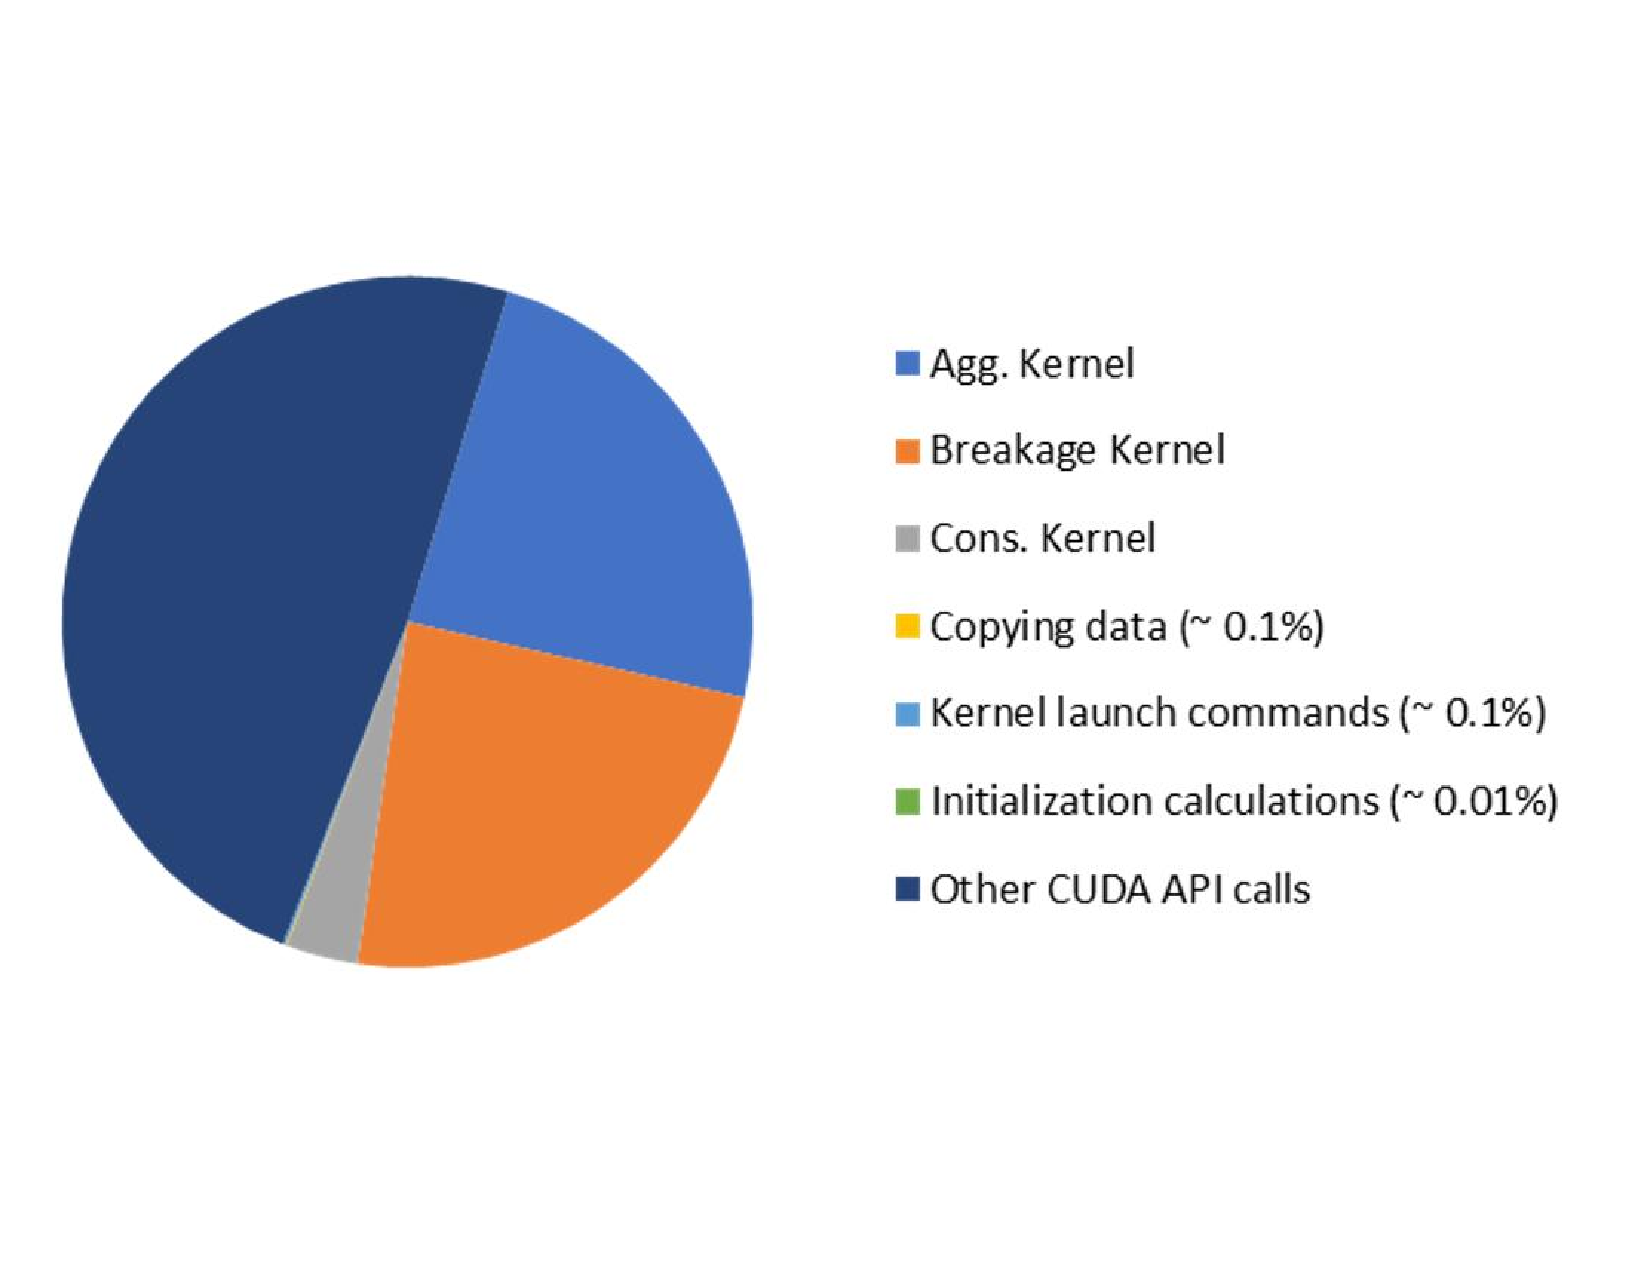
\includegraphics[scale=0.4]{Profile_Pie-converted.pdf}
\caption{Distribution of times taken by different processes inside the GPU-parallelized 
PBM}
\label{fig:res_profile_pie}
\end{figure}


\subsection{Performance on GPUs compared to CPUs}
The NVIDIA Quadro P4000 GPU used had its cores at a base clock speed of $1202$ MHz while
the CPU cores had a base clock of $4000$ MHz. The algorithm used to parallelize on the GPU 
did not permit the use of only one core of the GPU for simulation. Thus, a single MPI core 
CPU simulation was used as the baseline for all comparisons. Theoretically, it would take 
longer on a single core of the GPU to run a similar simulation than on a single GPU core

The CPU version of the parallel PBM was run on the desktop with the aforementioned 
configuration. This meant that the number of MPI cores available for the simulations 
was limited to 4. Soft scaling of the problem by changing the number of compartments 
was performed for this study. Figure \ref{fig:res_cpu_timings} shows a comparison of the times taken 
by the simulation to run on $1$, $2$ \& $4$ MPI cores. The times indicate that 
with the increase in the number of cores the model took less time to complete 
calculations for the same number of compartments. It can also be seen that for the 
same number of MPI cores used in a soft scaling the amount of time increases 
with increase in the number of cores. This increase can be attributed to the 
increase in the number of calculations with addition of new compartments. There is a 
slight plateau in the times when 2 and 4 MPI cores were used for $8$ and $16$ compartments 
respectively. When a further analysis of the rates was for each compartment was undertaken 
it was observed that till the particles did not each the last few compartments of the 
granulator the rates were $0$ thus reducing the compute time and leading to simulation
times in a similar range. 

\begin{figure}[h]
\centering
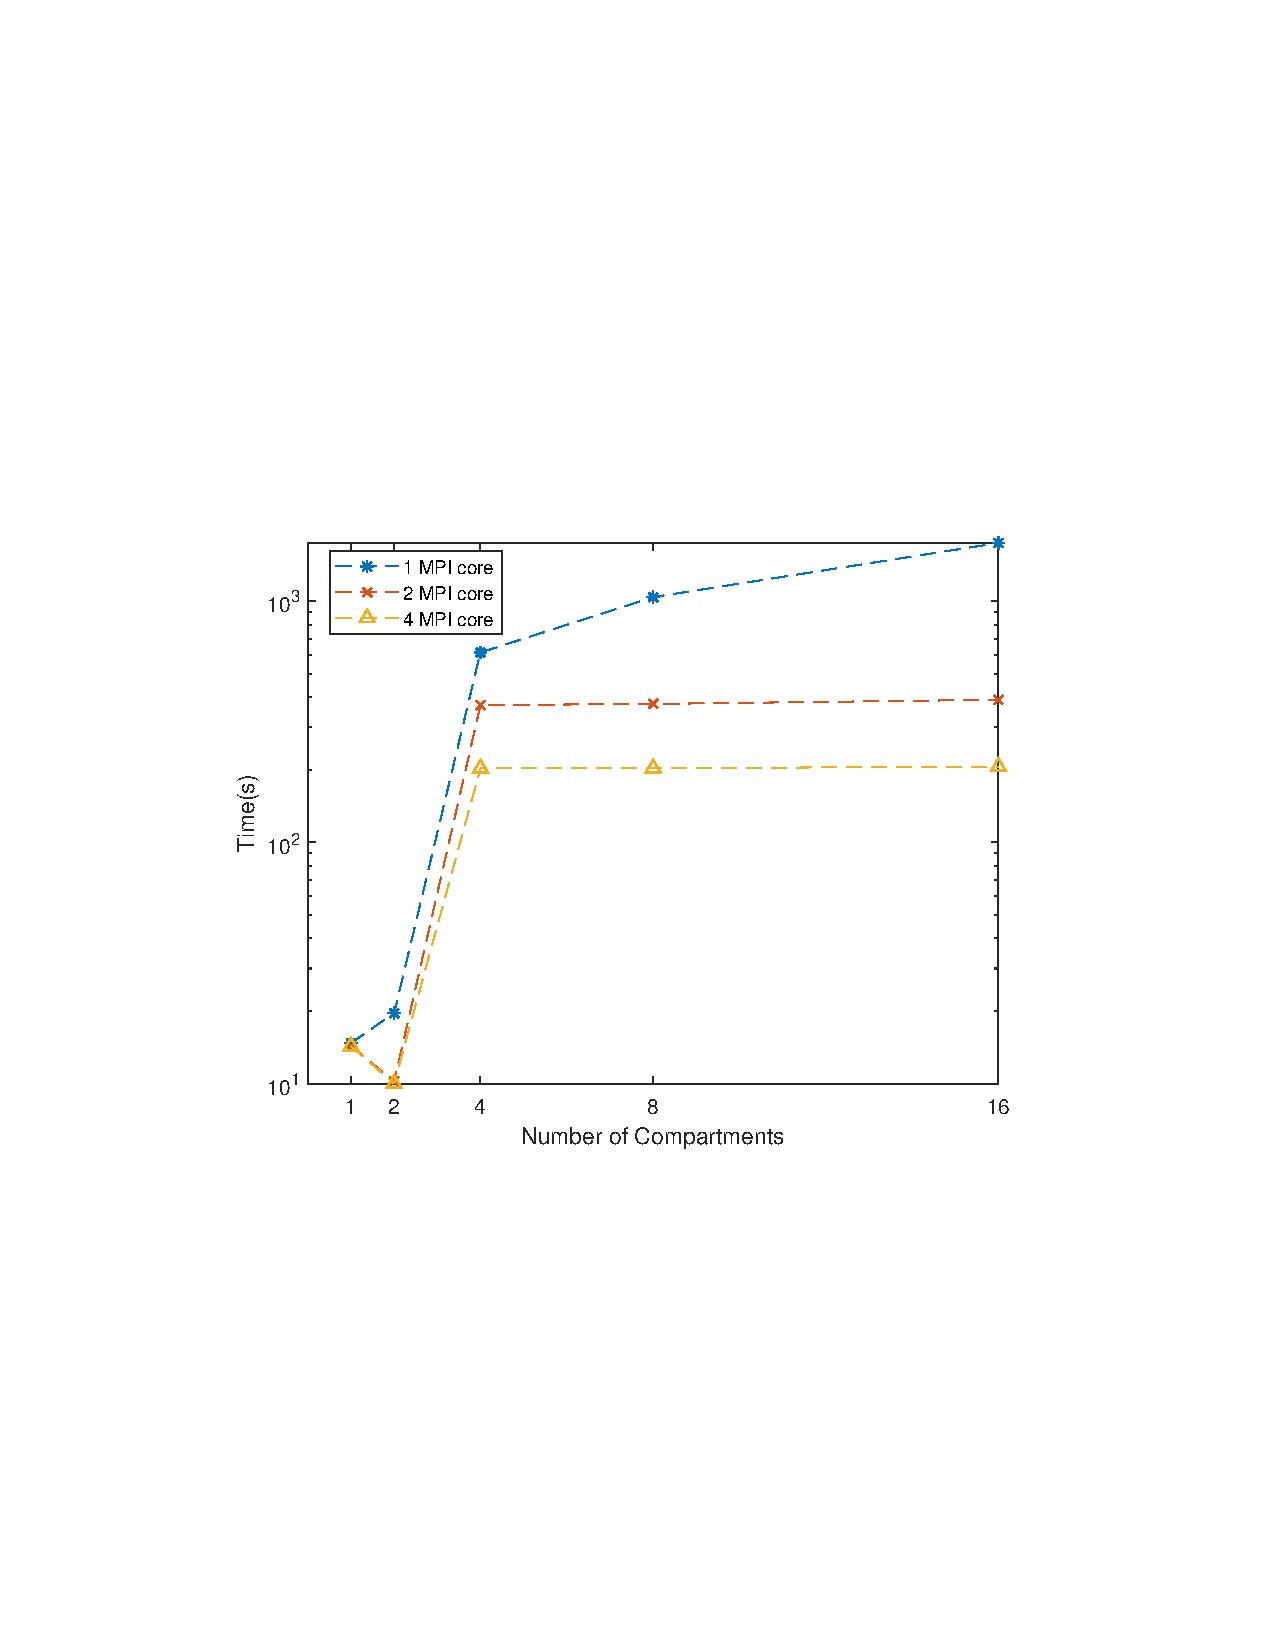
\includegraphics[scale=0.7,trim=100 240 100 240, clip]{cpu_desktopTiming.pdf}
\caption{Time taken to complete 90 seconds of PBM simulation with varying number of compartments 
on desktop CPU with varying number of MPI cores}
\label{fig:res_cpu_timings}
\end{figure}

Speedup is an important aspect that is considered to understand the scalability and 
parallel performance of a code. Speedup for a code is directly proportional 
to the number of cores used for a simulation. 
In Figure \ref{fig:res_desktop_speedup}, the speedup increases with the increase in 
the number of MPI cores. This increase in speedup can be attributed to the increase 
in the computation power. Another unusual trend observed in the case of 8, 16 and 
32 number of compartments, the speedup is higher than 2 and 4 for 2 MPI and 4 MPI core simulations respectively. This phenomena is known as super linear speedup which occurs 
when the speedup is greater than the number of cores used. In rare cases like these
speedup increases due to increase in cache memory and random access memory(RAM) 
available \citep{tuncer2009}. The simulations with the GPU parallel code showed an 
overall increase in the speedup as the number of compartments as seen in Figure 
\ref{fig:res_desktop_speedup}. The speedup was low for compartment numbers 1 and 2 
since the amount of time spent in communication in between the CPU and the GPU as well 
as the time taken by the SMs inside the GPU to distribute the problem had a larger 
contribution to the simulation time. The increase in number of compartments diminished 
this communication time effect as amount of calculations is significantly higher. The 
highest speeedup achieved for a GPU simulation was about $12.3$, which means it took 
$12$ times less time than a serial CPU computation. 


\begin{figure}[h]
\centering
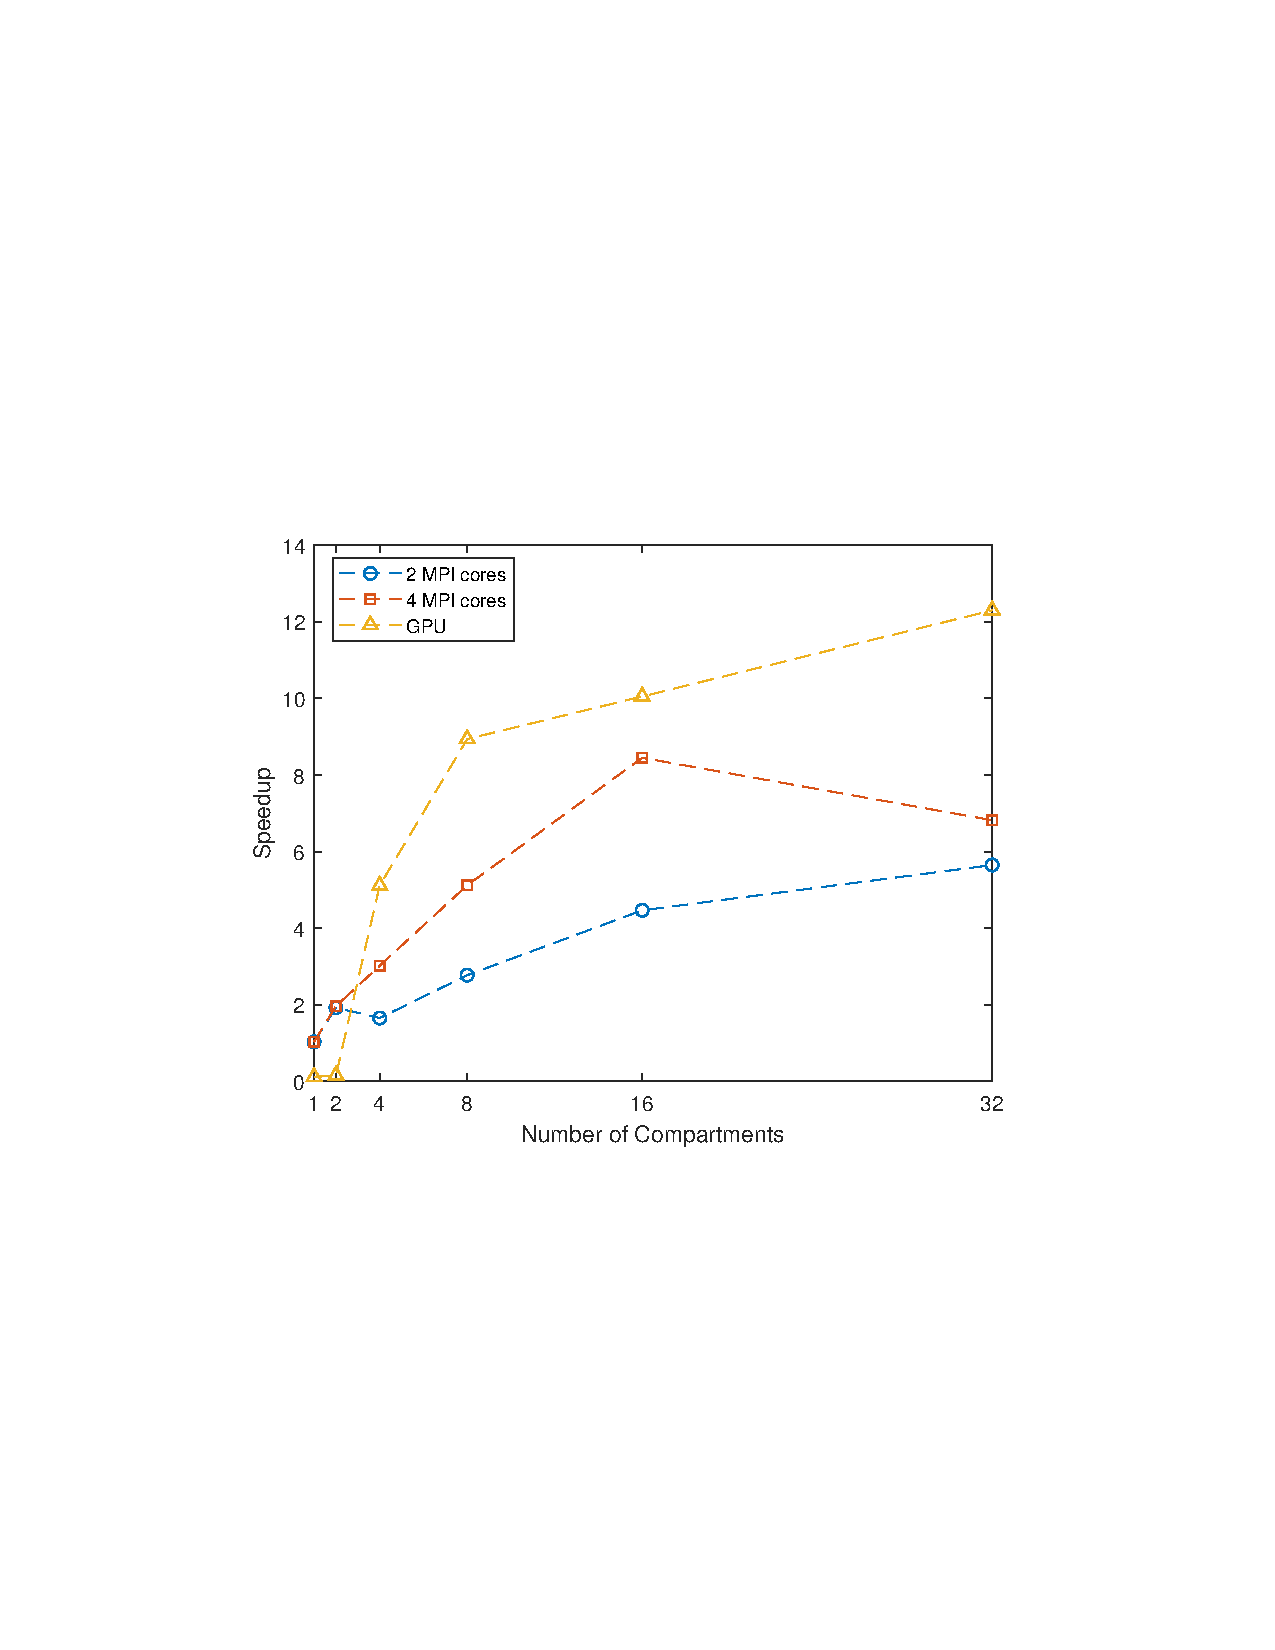
\includegraphics[scale=0.7,trim=120 240 120 240, clip]{speedup_desktop.pdf}
\caption{Comparing speedup for CPU and GPU simulations to respective serial simulations}
\label{fig:res_desktop_speedup}
\end{figure}



\subsection{Server level GPU code performance}
The high performance computing (HPC) device used to run the parallel PBM GPU code 
was present at Rutgers at the School of Engineering (SoE). The SoE HPC cluster was 
equipped with a NVIDIA Kepler K20 GPU. This GPU contains 2496 CUDA cores which are 
have a base clock of $706$ MHz and only 5 GB of GDDR5 of memory. The Kepler series 
GPUs were a couple of generations older than the Pascal generation Quadro P400 used 
in desktop simulation studies. The clock speed and memory of the desktop GPU was 
higher than the one present on the HPC. 

Time taken to complete the $90$ second PBM simulation on the HPC's GPU are shown in 
Figure \ref{fig:res_serverTimes}. The time taken to run the PBM initially remains 
constant upto 16 compartments, but a large increase in the time is observed for the 
simulation with 32 compartments. This increase could be attributed to the saturation 
of CUDA cores of the GPU and that SMs had to wait for the previous calculations to 
complete before the threads were assigned the remnant of calculations. A serial 
simulation was performed on the HPC and used as a baseline for speedup calculations. 
Speedup from the server GPUs are shown in Figure \ref{fig:res_serverSpeedup}. The 
increase in the speed of the simulation for these studies is lower than the desktop 
studies which could be directly connected to clock speeds of the CUDA cores. The 
server GPU cores were clocked at a lower frequency which meant the rate of calculations 
would decrease. One other reason for reduced speedup could be the older architecture 
of Kepler GPU which are slower in floating point calculations \citep{Pascal2016}.



\begin{figure}[H]
     \centering
     \begin{subfigure}[b]{0.48\linewidth}
         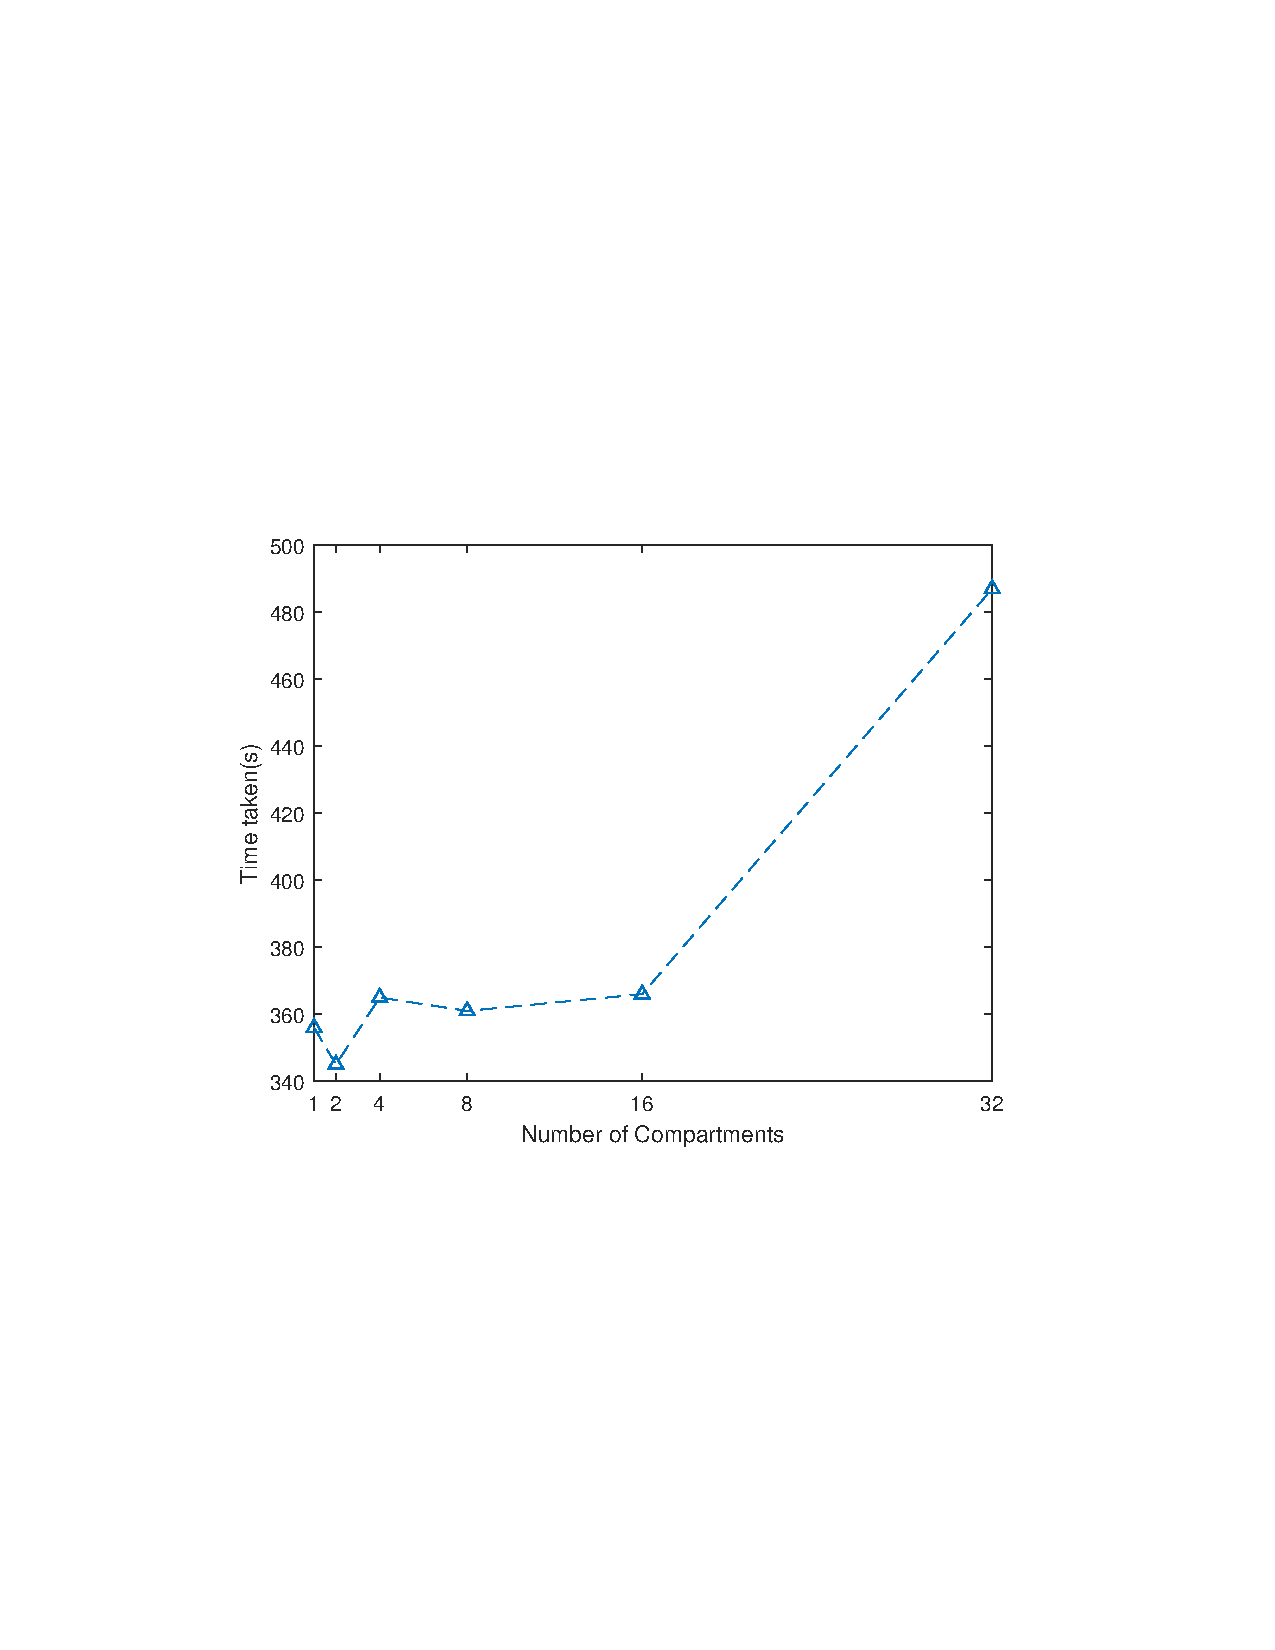
\includegraphics[scale=0.7,trim=120 240 120 240,width=\linewidth]{soe_gputimings.pdf}
         \caption{}
         \label{fig:res_serverTimes}
     \end{subfigure}
     \hfill
     \begin{subfigure}[b]{0.48\linewidth}
         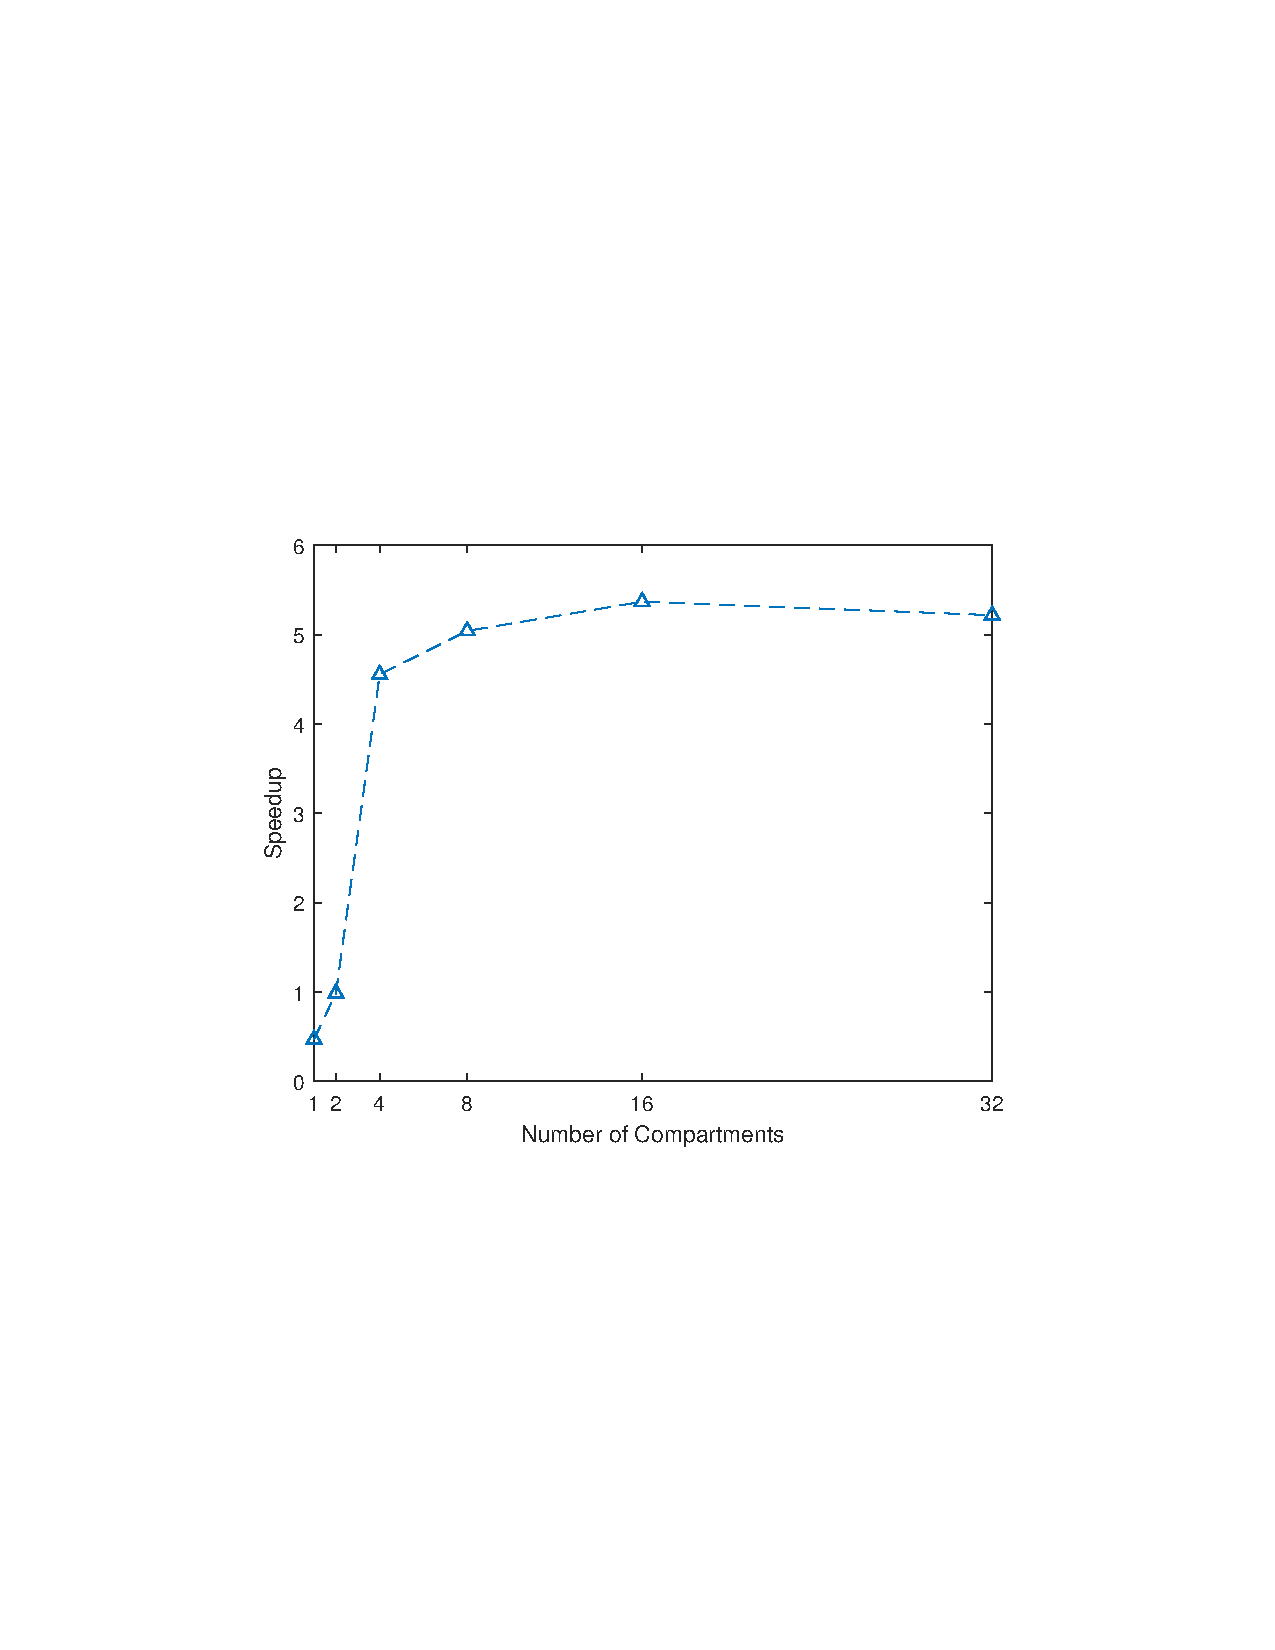
\includegraphics[scale=0.7,trim=120 240 120 240,width=\linewidth]{soe_gpuSpeedup.pdf}
         \caption{}
         \label{fig:res_serverSpeedup}
     \end{subfigure}
        \caption{(a)Time taken to run 90s PBM simulation on HPC's Kepler K20 GPU 
        (b)Speedup achieved for the GPU simulation over the serial simulation on the HPC device}
        \label{fig:res_server}
\end{figure}



\section{Conclusions}
\label{secConc}
In the presented study, a PBM was developed using to run parallel on a GPU. The time 
of the simulations on the GPU were compared to similar ones on CPUs. In most of the 
cases it was observed that GPU simulations were faster than CPU simulations where the 
problem size was large with minimal loss in accuracy. Simulations with low amounts 
of calculations were slower in case of GPUs, but such cases are rare in PBMs. 
The GPU architecture also plays a major role in the simulation. This work also 
highlighted that a desktop PC could be used for computationally intensive 
simulations rather than a supercomputer or cluster when resources are limited. 
This work can be extended in the future by testing on newer GPUs from NVIDIA 
like the Volta and Turing platforms, which are more optimized for float point calculations 
than the Pascal platform GPU used in this study. The algorithm to parallelize the code 
can also be parallelized further to eliminate loops inside the kernels using dynamic 
parallelization supported by newer versions of CUDA.

\appendix
\section{PBM model}
\label{app:A}
\subsection{Aggregation Kernel}
\label{app:aggKernel}

The aggregation kernel used in this work was formulated as in \cite{Barrasso2015ces}: 

\begin{align}
\beta(s_i,s_i',x)=C(s_i,s_i',x)\psi(s_i,s_i',x)
\label{eqn:mthds_pbm_beta_kernal}
\end{align}
The collision frequency of the solid particles was evaluated from the existing 
DEM data from \citep{Sampat2018}. To facilitate this study, it was assumed that
the collision frequency was independent of the liquid particles present in the 
system.

The collision efficiency $\psi$ was estimated based on Stokes , which 
states that a collision is successful when the Stokes number $St_v$ associated 
with the collision is lesser than the critical Stokes number ${St^*_v}$ for the 
particles. These number are calculated as follows:

\begin{align}
St_v=\frac{8\tilde{m}U}{3\pi\tilde{d^2}\mu}
\label{eqn:mthds_pbm_agg_Stnum}
\end{align}

\begin{align}
St^*_v=\left(1+\frac{1}{e}\right)log\left(\frac{h}{h_a}\right)
\label{eqn:mthds_pbm_agg_cricSt}
\end{align}
Here, $\tilde{m}$ \& $\tilde{d}$ represent the harmonic mean of the masses and 
diameters of the particles respectively.$U$ is the collision velocity, $\mu$ is the 
viscosity of the system and $e$ is the coefficient of restitution. The thickness of 
the liquid on the surface of the particle $h$ and the height of surface asperities 
$h_a$ were obtained from \citep{Barrasso2015ces}. $U_critical$ is defined as the 
ratio of the critical Stokes number to the Stokes number associated with the collision. 
The collision frequency $\psi$ is defined as:

\begin{align}
\Psi = \int_0^{U_critical} p(U)dU
\label{eqn:mthds_pbm_agg_psi}
\end{align}
where it is assumed that the collision velocities follow a log normal distribution:


\begin{align}
p(U) = \frac{1}{U\sqrt{2\pi}\sigma}\exp\left[-\frac{(lnU-\mu)^2}{2\sigma^2}\right]
\label{eqn:mthds_pbm_agg_lognormVelo}
\end{align}



\subsection{Breakage Kernel}
\label{app:breakKernel}
The breakage kernel $K_{break}(s_i,x)$ is formulated as: 

\begin{align}
K_{break}(s_i,x) = C_{impact}\int_{U_{break}}^{\infty}p(U)dU
\label{eqn:mthds_pbm_breakage_kernel}
\end{align}
Similar to the aggregation kernel, $C_impact$ is defined as rate at which 
the particles impact with the geometry in the DEM simulation. Critical velocity 
for breakage to occur is defined as:

\begin{align}
U_break=\frac{2St^*_def}{\rho_{s_i}}\frac{9}{8}\frac{(1-\epsilon)^2}{\epsilon}\frac{9\mu}{16d_{p_i}}
\label{eqn:mthds_pbm_breakage_ubreak}
\end{align}
where $2St^*_def$ is defined as critical Stokes deformation number \citep{Iveson2001} and 
$d_{p_i}$ is diameter of the solid particle $s_i$.



%\end{linenumbers}

\bibliographystyle{elsarticle-harv}
\bibliography{pbmGpuPaper}


\end{document}

%%
%% End of file `elsarticle-template-num.tex'.
